\documentclass[aspectratio=169,13pt,fleqn,t] {beamer}
%
% Choose how your presentation looks.
%
% For more themes, color themes and font themes, see:
% http://deic.uab.es/~iblanes/beamer_gallery/index_by_theme.html
%
\mode<presentation>
{
	\usetheme{Madrid}      % 整体主题
	\usecolortheme{beaver} % 配色主题（棕红系）
	\usefonttheme{serif}   % 全局衬线字体（正文宋体类）
	\setbeamertemplate{items}[default] % 【items父模板】控制 itemize+enumerate 符号
%	\setbeamertemplate{items}{\Large\beamertemplateballitem}
	\setbeamertemplate{sections/subsections in toc}[ball] % 目录里章节用圆圈标记
	
	%  \setbeamertemplate{navigation symbols}{} % 取消注释可隐藏底部导航小图标
	\setbeamertemplate{caption}[numbered] % 图/表标题带编号：图1、表1
}

\usepackage[,UTF8,linespread=1.2]{ctex}
\usepackage{wrapfig}
\usepackage{caption}
\usepackage{tcolorbox}
\tcbuselibrary{skins}
\captionsetup[figure]{name=图,labelsep=period}
\usepackage{pdfpages}
\usepackage{tabularx,array}
\usetikzlibrary{arrows.meta,intersections,positioning}

\usepackage{xcolor}
\definecolor{xy_blue}{cmyk}{0.6,0.35,0.0,0.4}
\definecolor{xy_orange}{cmyk}{0.0,0.7,1.0,0.0}
\definecolor{xy_green}{cmyk}{0.2,0.0,1.0,0.15}
\xdefinecolor{xy_gold}{RGB}{135,103,79}
\xdefinecolor{xy2_gold}{cmyk}{0,0.35,0.75,0.05}

\setbeamercolor{section number projected}{fg=red,bg=red!20}%控制球的颜色
\setbeamercolor{subsection number projected}{fg=blue,bg=blue!40}
\setbeamercolor{item}{fg=xy_gold} %设置列表项颜色

\usepackage{amsthm}
\newtheorem{peroration}{结论：}
\newtheorem*{exploration}{探究：}
\newtheorem*{prooft}{证明：}
\newtheorem*{solve}{解:} 
\newtheorem{instance}{例}   % 解：独立计数器
\newtheorem*{definate}{定义：}
     

% 配色（你前面需要的，每个环境单独颜色）
\setbeamercolor{theorem}{fg=black,bg=blue!10}
\setbeamercolor{solution}{fg=black,bg=green!10}

\BeforeBeginEnvironment{peroration}{%结论： 
	\setbeamercolor{block title}{bg=xy_green,fg=white}
	\setbeamercolor{block body}{bg=xy_green!10}
}
\AfterEndEnvironment{peroration}{
	\setbeamercolor{block title}{bg=xy_blue,fg=white}
	\setbeamercolor{block body}{bg=xy_blue!10}
}
\BeforeBeginEnvironment{exploration}{%探究
	\setbeamercolor{block title}{bg=xy_orange,fg=white}
	\setbeamercolor{block body}{bg=xy_orange!10}
}
\AfterEndEnvironment{peroration}{
	\setbeamercolor{block title}{bg=xy_blue,fg=white}
	\setbeamercolor{block body}{bg=xy_blue!10}
}
\BeforeBeginEnvironment{solution}{%解
	\begingroup
	\setbeamercolor{block title}{bg=xy_green,fg=white}
	\setbeamercolor{block body}{bg=xy_green!10}
}
\AfterEndEnvironment{solution}{
	\endgroup
}
\BeforeBeginEnvironment{prooft}{%证明
	\setbeamercolor{block title}{bg=xy_green,fg=white}
	\setbeamercolor{block body}{bg=xy_green!10}
}
\AfterEndEnvironment{prooft}{
	\setbeamercolor{block title}{bg=xy_green,fg=white}
	\setbeamercolor{block body}{bg=xy_green!10}
}
\BeforeBeginEnvironment{solve}{%解：
	\setbeamercolor{block title}{bg=xy_orange!60,fg=white}
	\setbeamercolor{block body}{bg=xy_orange!10}
}
\AfterEndEnvironment{solve}{%解：
	\setbeamercolor{block title}{bg=xy_orange!60,fg=white}
	\setbeamercolor{block body}{bg=xy_orange!10}
}
   
\BeforeBeginEnvironment{instance}{% 例子
	\begingroup
   	\setbeamercolor{block title}{bg=xy_gold!40,fg=white}
   	\setbeamercolor{block body}{bg=xy_gold!10}
   }
\AfterEndEnvironment{instance}{
	\endgroup
   }     
   
\renewcommand{\thefigure}{\arabic{figure}}

\title[含参数一元二次不等式的解法]{含参数一元二次不等式的解法}
\author[好好学习，努力向上]{}
\institute{}
\date{2026.10.08}
\setbeamertemplate{theorems}[numbered]

\AtBeginSection[]
{
  \begin{frame}<beamer>
    \frametitle{本节主要内容概览}
    \tableofcontents[currentsection,currentsubsection]
  \end{frame}
}

\begin{document}
\begin{frame}{}
	\titlepage
\end{frame}

\begin{frame}{本节主要内容概览}
	\tableofcontents
\end{frame}

\section{前情回顾}
\begin{frame}{解一元二次不等式的程序}
	
	\vspace{-1em}
	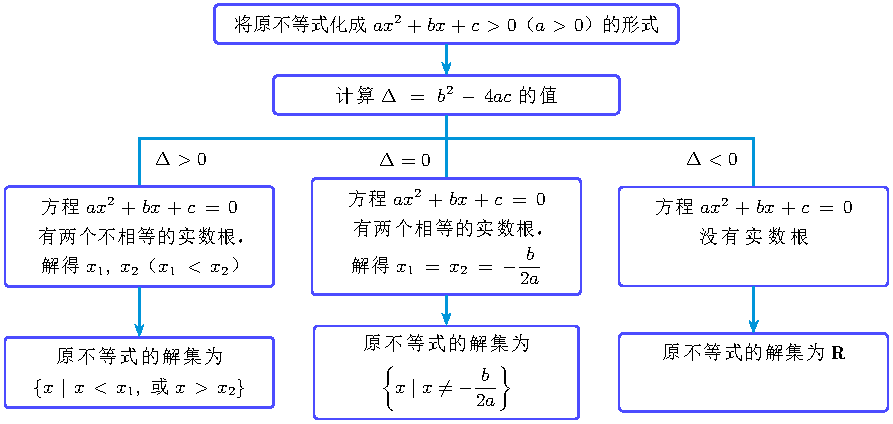
\includegraphics{Figures/budengshi7.pdf}
	
\end{frame}



\begin{frame}[t]{一元二次不等式与二次函数、一元二次方程的关系}
	\small
	\begin{tabularx}{\textwidth}[c]{|*{4}{>{\arraybackslash}m{3.37cm}|}}
		\hline
		\centering 项目 &	\centering $\Delta>0$	& \centering$\Delta=0$	&	\centering\arraybackslash$\Delta<0$	\\
		\hline
		$y=ax^2+bx+c(a>0)$的图象	&	
		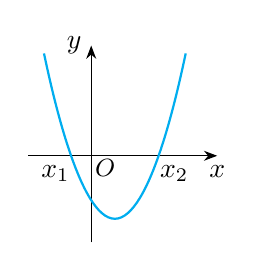
\begin{tikzpicture}[baseline={(0,-1)}]
			\draw[-Stealth,name path=line](-0.8,0) -- (1.6,0)node[below]{$x$};
			\draw[-Stealth](0,-1.1) -- (0,1.4)node[left]{$y$};
			\draw[thick,cyan,name path=curve](-0.6,1.3) parabola bend(0.3,-0.8) (1.2,1.3);
			\path[name intersections={of= line and curve,name=t}]
			(t-1)node[below left= 0pt and  -3pt]{$x_1$}
			(t-2)node[below right= 0pt and  -3pt]{$x_2$};
			\node[below right=-3pt] at (0,0){\small $O$};
		\end{tikzpicture}	&	
		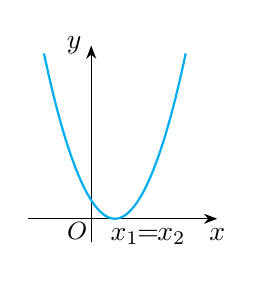
\begin{tikzpicture}[baseline={(0,-1)}]
			\draw[-Stealth,name path=line](-0.8,-0.8) -- (1.6,-0.8)node[below]{$x$};
			\draw[-Stealth](0,-1.1) -- (0,1.4)node[left]{$y$};
			\draw[thick,cyan,name path=curve](-0.6,1.3) parabola bend(0.3,-0.8) (1.2,1.3);
			\path[name intersections={of= line and curve,name=t}]
			(t-1)node[below right =0pt and -5pt ]{$x_1\!\!=\!\! x_2$};
			\node[below left=-3pt] at(0,-0.8){\small $O$};			
		\end{tikzpicture}		&	
		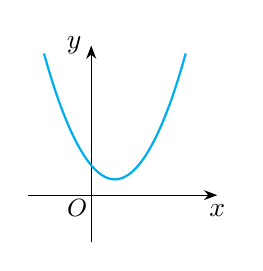
\begin{tikzpicture}[baseline={(0,-1)}]
			\draw[-Stealth,name path=line](-0.8,-0.5) -- (1.6,-0.5)node[below]{$x$};
			\draw[-Stealth](0,-1.1) -- (0,1.4)node[left]{$y$};
			\draw[thick,cyan,name path=curve](-0.6,1.3) parabola bend(0.3,-0.3) (1.2,1.3);			
			\node[below left=-3pt] at(0,-0.5){\small $O$};			
		\end{tikzpicture}	\\
		\hline
		$ax^2+bx+c=0(a>0)$的根	&	有两个不相等的实数根$x_1,x_2(x_1<x_2)$	&	有两个相等的实数根$x_1=x_2=-\frac{b}{2a}$	&	没有实数根	\\
		\hline
		$ax^2+bx+c>0(a\neq 0)$的根	&$\{x\mid x<x_1,\text{或} x>x_2\}$	&	$\{x\mid x \neq -\frac{b}{2a}\}$	&	\centering\arraybackslash$\mathbf{R}$		\\
		\hline
		$ax^2+bx+c<0(a>0)$的解集	&	\centering$\{x \mid x_1<x<x_2\}$		&	\centering$\varnothing$	&	\centering\arraybackslash$\varnothing$	\\
		\hline
	\end{tabularx}


\end{frame}

\section{例题分析}
\begin{frame}[<+->]{例题分析}
	\vspace{-1.5em}


\begin{instance}
	求不等式$x^2 - x + m(1-m) > 0$的解集。
\end{instance}

\begin{solve}
	

将不等式左边因式分解：
\[
x^2 - x + m(1-m) = (x-m)(x + m - 1)
\]
原不等式等价于：
\[
(x-m)[x - (1-m)] > 0
\]
对应方程的两个根为 \(x_1 = m\) 和 \(x_2 = 1 - m\)。
\end{solve}
\end{frame}

\begin{frame}{}
	
\begin{solve}[接上页]
	

比较两个根的大小：
\begin{enumerate}[(1)]
	\item 令 \(m = 1 - m\)，解得 \(m = \frac{1}{2}\)。
	\item 令 \(m > 1 - m\)，解得 \(m > \frac{1}{2}\)。
	\item 令 \(m < 1 - m\)，解得 \(m < \frac{1}{2}\)。
\end{enumerate}

根据根的大小关系，分情况写出解集（大于取两边）：

\begin{enumerate}[(1)]
	\item \textbf{当 \(m > \frac{1}{2}\) 时，\(m > 1-m\)：}
	解集为 \(\{x \mid x < 1-m \text{ 或 } x > m\}\)。
	
	\item \textbf{当 \(m = \frac{1}{2}\) 时，\(m = 1-m = \frac{1}{2}\)：}
	不等式变为 \((x - \frac{1}{2})^2 > 0\)。
	解集为 \(\{x \mid x \neq \frac{1}{2}\}\)。
	
	\item \textbf{当 \(m < \frac{1}{2}\) 时，\(m < 1-m\)：}
	解集为 \(\{x \mid x < m \text{ 或 } x > 1-m\}\)。
\end{enumerate}
\end{solve}
\end{frame}

\begin{frame}{例题分析}
	\vspace{-1.5em}
\begin{instance}<1->
	求不等式$x^2 - 2mx + (m+2) < 0$的解集。
\end{instance}
	\vspace{-1em}
	\begin{solve}<2->		
		考虑对应的一元二次方程 \(x^2 - 2mx + (m+2) = 0\)。
		其判别式 \(\Delta = (-2m)^2 - 4 \times 1 \times (m+2) = 4m^2 - 4m - 8 = 4(m^2 - m - 2) = 4(m-2)(m+1)\)。
		
		根据判别式的符号，我们分情况讨论：
		
		\begin{enumerate}[(1)]
			\item \textbf{当 \(\Delta < 0\) 时，即 \(-1 < m < 2\) 时：}
			抛物线开口向上且与 \(x\) 轴无交点，不等式 \(x^2 - 2mx + (m+2) < 0\) 无解。
			此时解集为 \(\varnothing\)。
			
			\item \textbf{当 \(\Delta = 0\) 时，即 \(m = -1\) 或 \(m = 2\) 时：}
			方程有两个相等的实根。
			\begin{itemize}
				\item 若 \(m = -1\)，方程为 \(x^2 + 2x + 1 = 0\)，即 \((x+1)^2 = 0\)，根为 \(x = -1\)。不等式 \((x+1)^2 < 0\) 无解，解集为 \(\varnothing\)。
				\item 若 \(m = 2\)，方程为 \(x^2 - 4x + 4 = 0\)，即 \((x-2)^2 = 0\)，根为 \(x = 2\)。不等式 \((x-2)^2 < 0\) 无解，解集为 \(\varnothing\)。
			\end{itemize}
			
		\end{enumerate}
	\end{solve}
\end{frame}

\begin{frame}{}
	\begin{solve}[接上页]
		
		\begin{enumerate}[(3)]
	\setcounter{enumi}{2}
			\item \textbf{当 \(\Delta > 0\) 时，即 \(m < -1\) 或 \(m > 2\) 时：}
		方程有两个不相等的实根，由求根公式得：
		\[
		x = \frac{2m \pm \sqrt{4(m-2)(m+1)}}{2} = m \pm \sqrt{m^2 - m - 2}
		\]
		因为抛物线开口向上，不等式的解集在两根之间。
		此时解集为 \(\{x \mid m - \sqrt{m^2 - m - 2} < x < m + \sqrt{m^2 - m - 2}\}\)。
		\end{enumerate}
			\textbf{综上所述：}
		\begin{enumerate}[(1)]
			\item 当 \(-1 \le m \le 2\) 时，解集为 \(\varnothing\)；
			\item 当 \(m < -1\) 或 \(m > 2\) 时，解集为 \((m - \sqrt{m^2 - m - 2}, m + \sqrt{m^2 - m - 2})\)。
		\end{enumerate}
	\end{solve}
	
\end{frame}

\begin{frame}{例题分析}
	\vspace{-1.5em}
	\begin{instance}<1->
		已知不等式$x^2 + mx + n < 0$的解集为$\{x \;\mid \;1 < x < 4\}$，
		\begin{enumerate}[(1)]
			\item 求$m$和$n$的值。
			\item 若$x^2 + mx + n \leqslant ax$对一切$x > 0$恒成立，求实数$a$的取值范围。
		\end{enumerate}
	\end{instance}
	\vspace{-1em}
	\begin{solve}<2->		
(1)	由题意知，不等式 \(x^2 + mx + n < 0\) 的解集为 \((1, 4)\)。
	这说明二次方程 \(x^2 + mx + n = 0\) 的两个根分别为 \(x_1 = 1\) 和 \(x_2 = 4\)。
	
	根据韦达定理（根与系数的关系）：
	\begin{align*}
		x_1 + x_2 &= -m \implies 1 + 4 = -m \implies m = -5 \\
		x_1 \cdot x_2 &= n \implies 1 \times 4 = n \implies n = 4
	\end{align*}
	所以，\(m = -5\)，\(n = 4\)。
	\end{solve}
\end{frame}

\begin{frame}{}
	\begin{solve}[接上页]
(2)		由 (1) 知，不等式为 \(x^2 - 5x + 4 \le ax\)。

		整理得：\(x^2 - (5+a)x + 4 \le 0\)。
		该不等式对一切 \(x > 0\) 恒成立。
		
		由于 \(x > 0\)，我们可以将不等式两边同时除以 \(x\)，得：
		\[
		x - (5+a) + \frac{4}{x} \le 0
		\]
		\[
		x + \frac{4}{x} \le 5 + a
		\]
		要使该不等式对一切 \(x > 0\) 恒成立，只需 \(5+a\) 大于等于函数 \(f(x) = x + \frac{4}{x}\) 在 \(x > 0\) 时的最小值。
		
	\end{solve}
\end{frame}
\begin{frame}
	\begin{solve}[接上页]
		根据基本不等式：
		\[
		x + \frac{4}{x} \ge 2\sqrt{x \cdot \frac{4}{x}} = 2\sqrt{4} = 4
		\]
		当且仅当 \(x = \frac{4}{x}\)，即 \(x = 2\) 时（满足 \(x>0\)），等号成立。
		所以，\(f(x)\) 的最小值为 \(4\)。
		
		因此，我们只需要：
		\[
		5 + a \ge 4
		\]
		\[
		a \ge -1
		\]
		
		所以，实数 \(a\) 的取值范围是 \([-1, +\infty)\)。
	\end{solve}
\end{frame}



\begin{frame}[t]{小结：解含参数一元二次不等式的方法步骤：}
	\begin{enumerate}
		\item 解相应的一元二次方程，求方程的根
		\item 比较方程的根的大小，写出一元二次不等式的解集
	\end{enumerate}

\end{frame}

\end{document}
